% ===== 薄透镜焦距三种测量方法 实验报告 =====
% 姓名：叶哲昊  学号：24012561  实验日期：2026年5月15日
\documentclass[12pt, a4paper]{article}

% ===== 中文支持 =====
\usepackage[UTF8, zihao=-4]{ctex}

% ===== 页边距（GB/T 7713.1） =====
\usepackage[top=2.5cm, bottom=2.5cm, left=2.8cm, right=2.8cm]{geometry}

% ===== 字体 =====
\usepackage{fontspec}
\setmainfont{Times New Roman}

% ===== 行距 =====
\usepackage{setspace}
\setstretch{1.5}
\setlength{\parskip}{0pt}

% ===== 插图 =====
\usepackage{graphicx}
\usepackage{float}
\graphicspath{{./}}

% ===== 表格 =====
\usepackage{booktabs}
\usepackage{array}
\usepackage{makecell}
\usepackage{multirow}
\usepackage{adjustbox}

% ===== 数学 =====
\usepackage{amsmath, amssymb}

% ===== 图表编号（章-序号） =====
\usepackage{chngcntr}
\renewcommand{\thefigure}{\arabic{section}-\arabic{figure}}
\renewcommand{\thetable}{\arabic{section}-\arabic{table}}
\counterwithin{figure}{section}
\counterwithin{table}{section}

% ===== 图表标题格式 =====
\usepackage{caption}
\captionsetup{font=small, labelsep=space, justification=centering,
              aboveskip=6pt, belowskip=12pt}
\captionsetup[table]{aboveskip=12pt, belowskip=6pt, position=above}

% ===== 页眉页脚 =====
\usepackage{fancyhdr}
\setlength{\headheight}{15pt}
\pagestyle{fancy}
\fancyhf{}
\fancyhead[C]{\small 实验报告——薄透镜焦距三种测量方法}
\fancyfoot[C]{\small\thepage}

% ===== 章节标题格式 =====
\usepackage{titlesec}
\titleformat{\section}[block]
  {\centering\heiti\zihao{4}}{\thesection}{1em}{}
\titlespacing*{\section}{0pt}{24pt}{18pt}
\titleformat{\subsection}[hang]
  {\heiti\zihao{-4}}{\thesubsection}{1em}{}
\titlespacing*{\subsection}{0pt}{18pt}{6pt}
\titleformat{\subsubsection}[hang]
  {\heiti\zihao{-4}}{\thesubsubsection}{1em}{}
\titlespacing*{\subsubsection}{0pt}{12pt}{6pt}

% ===== 超链接 =====
\usepackage[colorlinks=true, linkcolor=black, citecolor=black,
            urlcolor=blue, bookmarks=true]{hyperref}

\begin{document}

% ===== 封面 =====
\begin{titlepage}
  \centering
  \vspace*{3cm}
  {\heiti\zihao{2} 实验报告} \\[1cm]
  {\heiti\zihao{3} 薄透镜焦距三种测量方法} \\[2cm]
  \begin{tabular}{ll}
    姓\quad 名：   & 叶哲昊 \\[0.5cm]
    学\quad 号：   & 24012561 \\[0.5cm]
    实验日期：     & 2026 年 5 月 15 日 \\
  \end{tabular}
  \vfill
\end{titlepage}

\tableofcontents
\newpage
\setcounter{page}{1}

% ========== 第 1 节：实验目的 ==========
\section{实验目的}

\begin{enumerate}
  \item 学会调节光学系统共轴，掌握光学元件在导轨上的正确安装与调试方法。
  \item 掌握薄透镜焦距的常用测量方法：自准直法与二次成像法（贝塞尔法）。
  \item 研究透镜成像规律，理解共轭点（物像对称）的概念。
  \item 通过多次测量与数据处理，掌握直接测量量的误差分析方法。
\end{enumerate}

% ========== 第 2 节：实验原理 ==========
\section{实验原理}

\subsection{自准直法}

自准直法（auto-collimation method）是光学实验中常用的方法，利用平行光经平面反射镜
反射后原路返回成像的原理来确定透镜焦距。

如图~\ref{fig:zizhi-principle} 所示，若物体 $AB$ 恰好处于凸透镜 $L$ 的前焦面处，则物体各点
发出的光经透镜折射后变为不同方向的平行光束；该平行光束经后方的平面反射镜 $M$ 全反射
后，再次通过透镜，最终在原物平面处形成倒立、与原物等大的实像 $A'B'$。此时，物体到
透镜的距离即为透镜焦距 $f$，可直接由光学导轨的刻度读出：
\begin{equation}
  f = a_2 - a_1 \label{eq:zizhi}
\end{equation}
其中 $a_1$ 为目标板在导轨上的位置读数，$a_2$ 为待测透镜的位置读数（实验中透镜位于目标板右侧，故 $a_2 > a_1$）。

\begin{figure}[H]
  \centering
  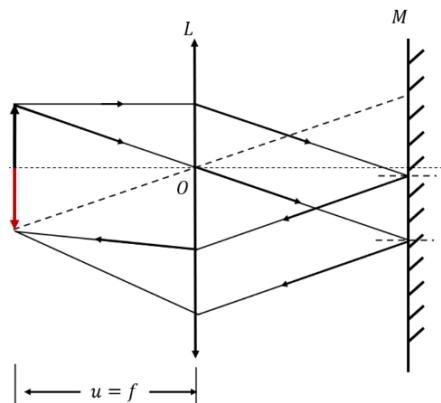
\includegraphics[width=0.65\textwidth]{images/5bd946e29cc0ed8bfbfc30f7c5d75507c460243a085f4207594b597d5bd533a5.jpg}
  \caption{自准直法测凸透镜焦距原理图}
  \label{fig:zizhi-principle}
\end{figure}

\subsection{二次成像法（贝塞尔法）}

二次成像法（Bessel method，又称贝塞尔法）利用透镜成像的共轭对称性，通过两次清晰
成像来计算焦距，无需考虑透镜的主平面位置，因此测量精度较高。

如图~\ref{fig:bessel-principle} 所示，当物体与光屏之间的距离 $l > 4f'$ 时，保持二者位置
不变，在物与屏之间移动凸透镜，可以找到两个使屏上成清晰像的透镜位置；设两个位置之
间的距离为 $d$，利用物像的共轭对称性，可以证明：
\begin{equation}
  f' = \frac{l^2 - d^2}{4l} \label{eq:bessel}
\end{equation}
其中 $d = a_2 - a_1$，$a_1$、$a_2$ 分别为两次清晰成像时透镜的导轨位置读数，$l$ 为目标
板（物）到白屏（像面）的距离。

\begin{figure}[H]
  \centering
  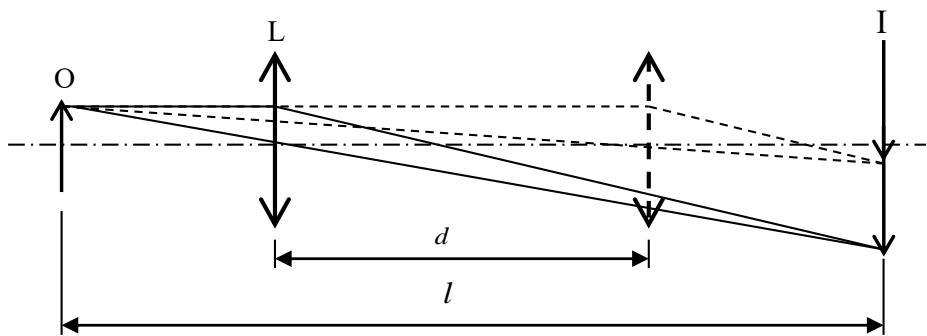
\includegraphics[width=0.65\textwidth]{images/cadc91086c8355ab655ac4a9f435530095076a2197ba5276d3af1f965c94812a.jpg}
  \caption{二次成像法（贝塞尔法）测凸透镜焦距原理图}
  \label{fig:bessel-principle}
\end{figure}

\subsection{平行光管法}

平行光管（collimator）是一种利用分划板置于物镜焦平面上、使光源成为等效无穷远目标
的仪器。平行光管法根据分划板像的大小 $y'$ 及分划板实际尺寸 $y$，结合平行光管物镜焦距
$f_o'$，由下式计算待测透镜焦距：
\begin{equation}
  f_x' = \frac{y'}{y} f_o' \label{eq:collimator}
\end{equation}
本次实验由于相关设备（CMOS 相机及配套焦距测量软件）不具备使用条件，平行光管法
未能实施，故本报告仅含自准直法与二次成像法的实验数据与结果。

% ========== 第 3 节：实验仪器 ==========
\section{实验仪器}

\begin{enumerate}
  \item 光学导轨（带刻度尺，精度 $1\,\text{mm}$）及导轨滑块若干。
  \item "F"形 LED 光源（目标板），作为物体。
  \item 待测凸透镜一：$\Phi 50\,\text{mm}$，标称焦距 $f = 200\,\text{mm}$（用于自准直法）。
  \item 待测凸透镜二：$\Phi 50\,\text{mm}$，标称焦距 $f = 150\,\text{mm}$（用于二次成像法）。
  \item 平面反射镜（用于自准直法）。
  \item 白屏（用于二次成像法）。
  \item 钢直尺（辅助测量物屏间距）。
\end{enumerate}

% ========== 第 4 节：实验步骤 ==========
\section{实验步骤}

\subsection{共轴调节}

在进行各项测量之前，先进行共轴调节：将所有光学元件安装于导轨上，由近及远逐步调节
各元件的高度与横向位置，使"F"形光斑始终通过透镜光心；对正方向后，固定各元件。

\subsection{自准直法测焦距}

\begin{enumerate}
  \item 依次将 LED 光源、待测透镜（标称 $200\,\text{mm}$）、平面反射镜安装于导轨上（图~\ref{fig:zizhi-photo}）。
  \item 使"F"形光斑入射到透镜中心；紧靠透镜后安装平面反射镜，调整反射镜角度使反射光斑与物同高。
  \item 同时平移透镜与反射镜，直至目标板上出现清晰、与物等大、轮廓为长方形的倒立实像。
  \item 分别记录目标板位置 $a_1$（mm）和透镜位置 $a_2$（mm），按式~(\ref{eq:zizhi}) 计算 $f$。
  \item 重复上述调节 3 次，取平均值。
\end{enumerate}

\begin{figure}[H]
  \centering
  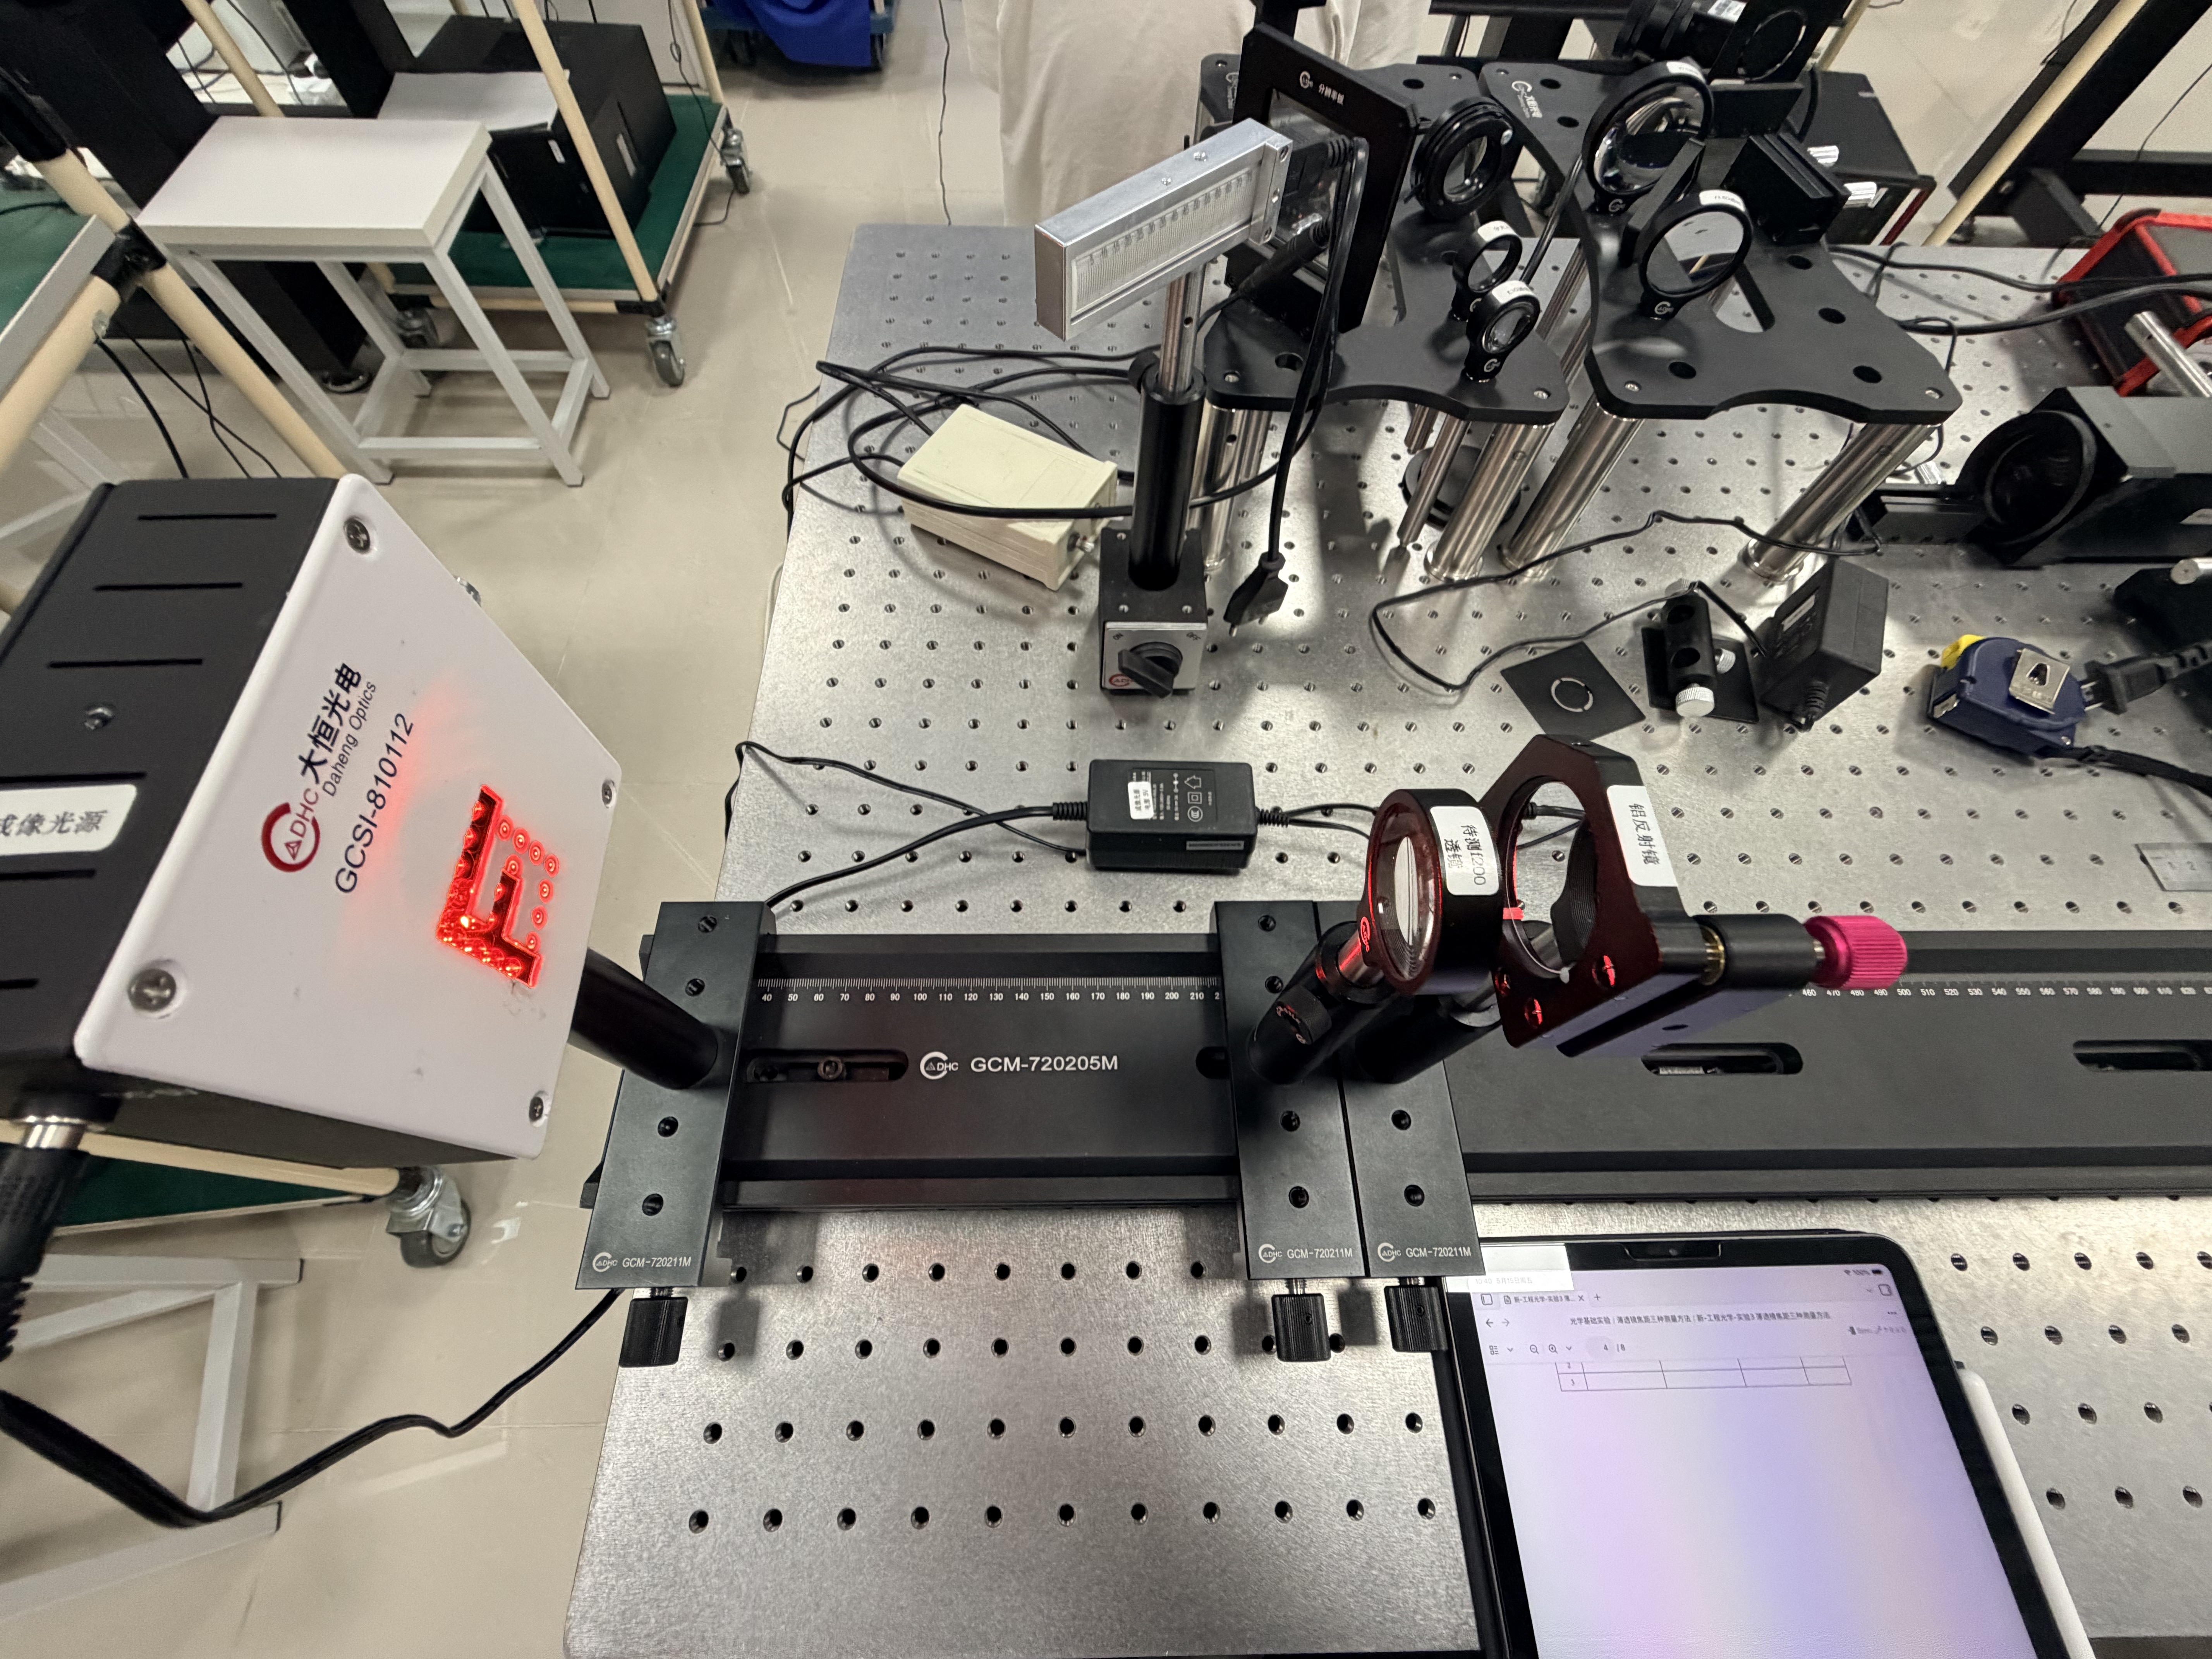
\includegraphics[width=0.7\textwidth]{实验照片/自准直法光路照片.jpg}
  \caption{自准直法实验光路（实拍）}
  \label{fig:zizhi-photo}
\end{figure}

\subsection{二次成像法（贝塞尔法）测焦距}

\begin{enumerate}
  \item 依次将 LED 光源、待测透镜（标称 $150\,\text{mm}$）、白屏安装于导轨上。
  \item 调整白屏与目标板之间的距离 $l \geq 600\,\text{mm}$（满足 $l > 4f'$ 的条件）。
  \item 从目标板一侧向白屏方向缓慢移动透镜，找到第一个使白屏上像清晰的位置，记录透镜
        导轨读数 $a_1$（图~\ref{fig:bessel-a1}）。
  \item 继续向白屏方向移动透镜，找到第二个清晰位置，记录 $a_2$（图~\ref{fig:bessel-a2}）。
  \item 测量目标板到白屏的间距 $l$，按式~(\ref{eq:bessel}) 计算 $f'$。
  \item 重复上述操作 3 次（改变物屏距），取平均值。
\end{enumerate}

\begin{figure}[H]
  \centering
  \begin{minipage}[b]{0.48\textwidth}
    \centering
    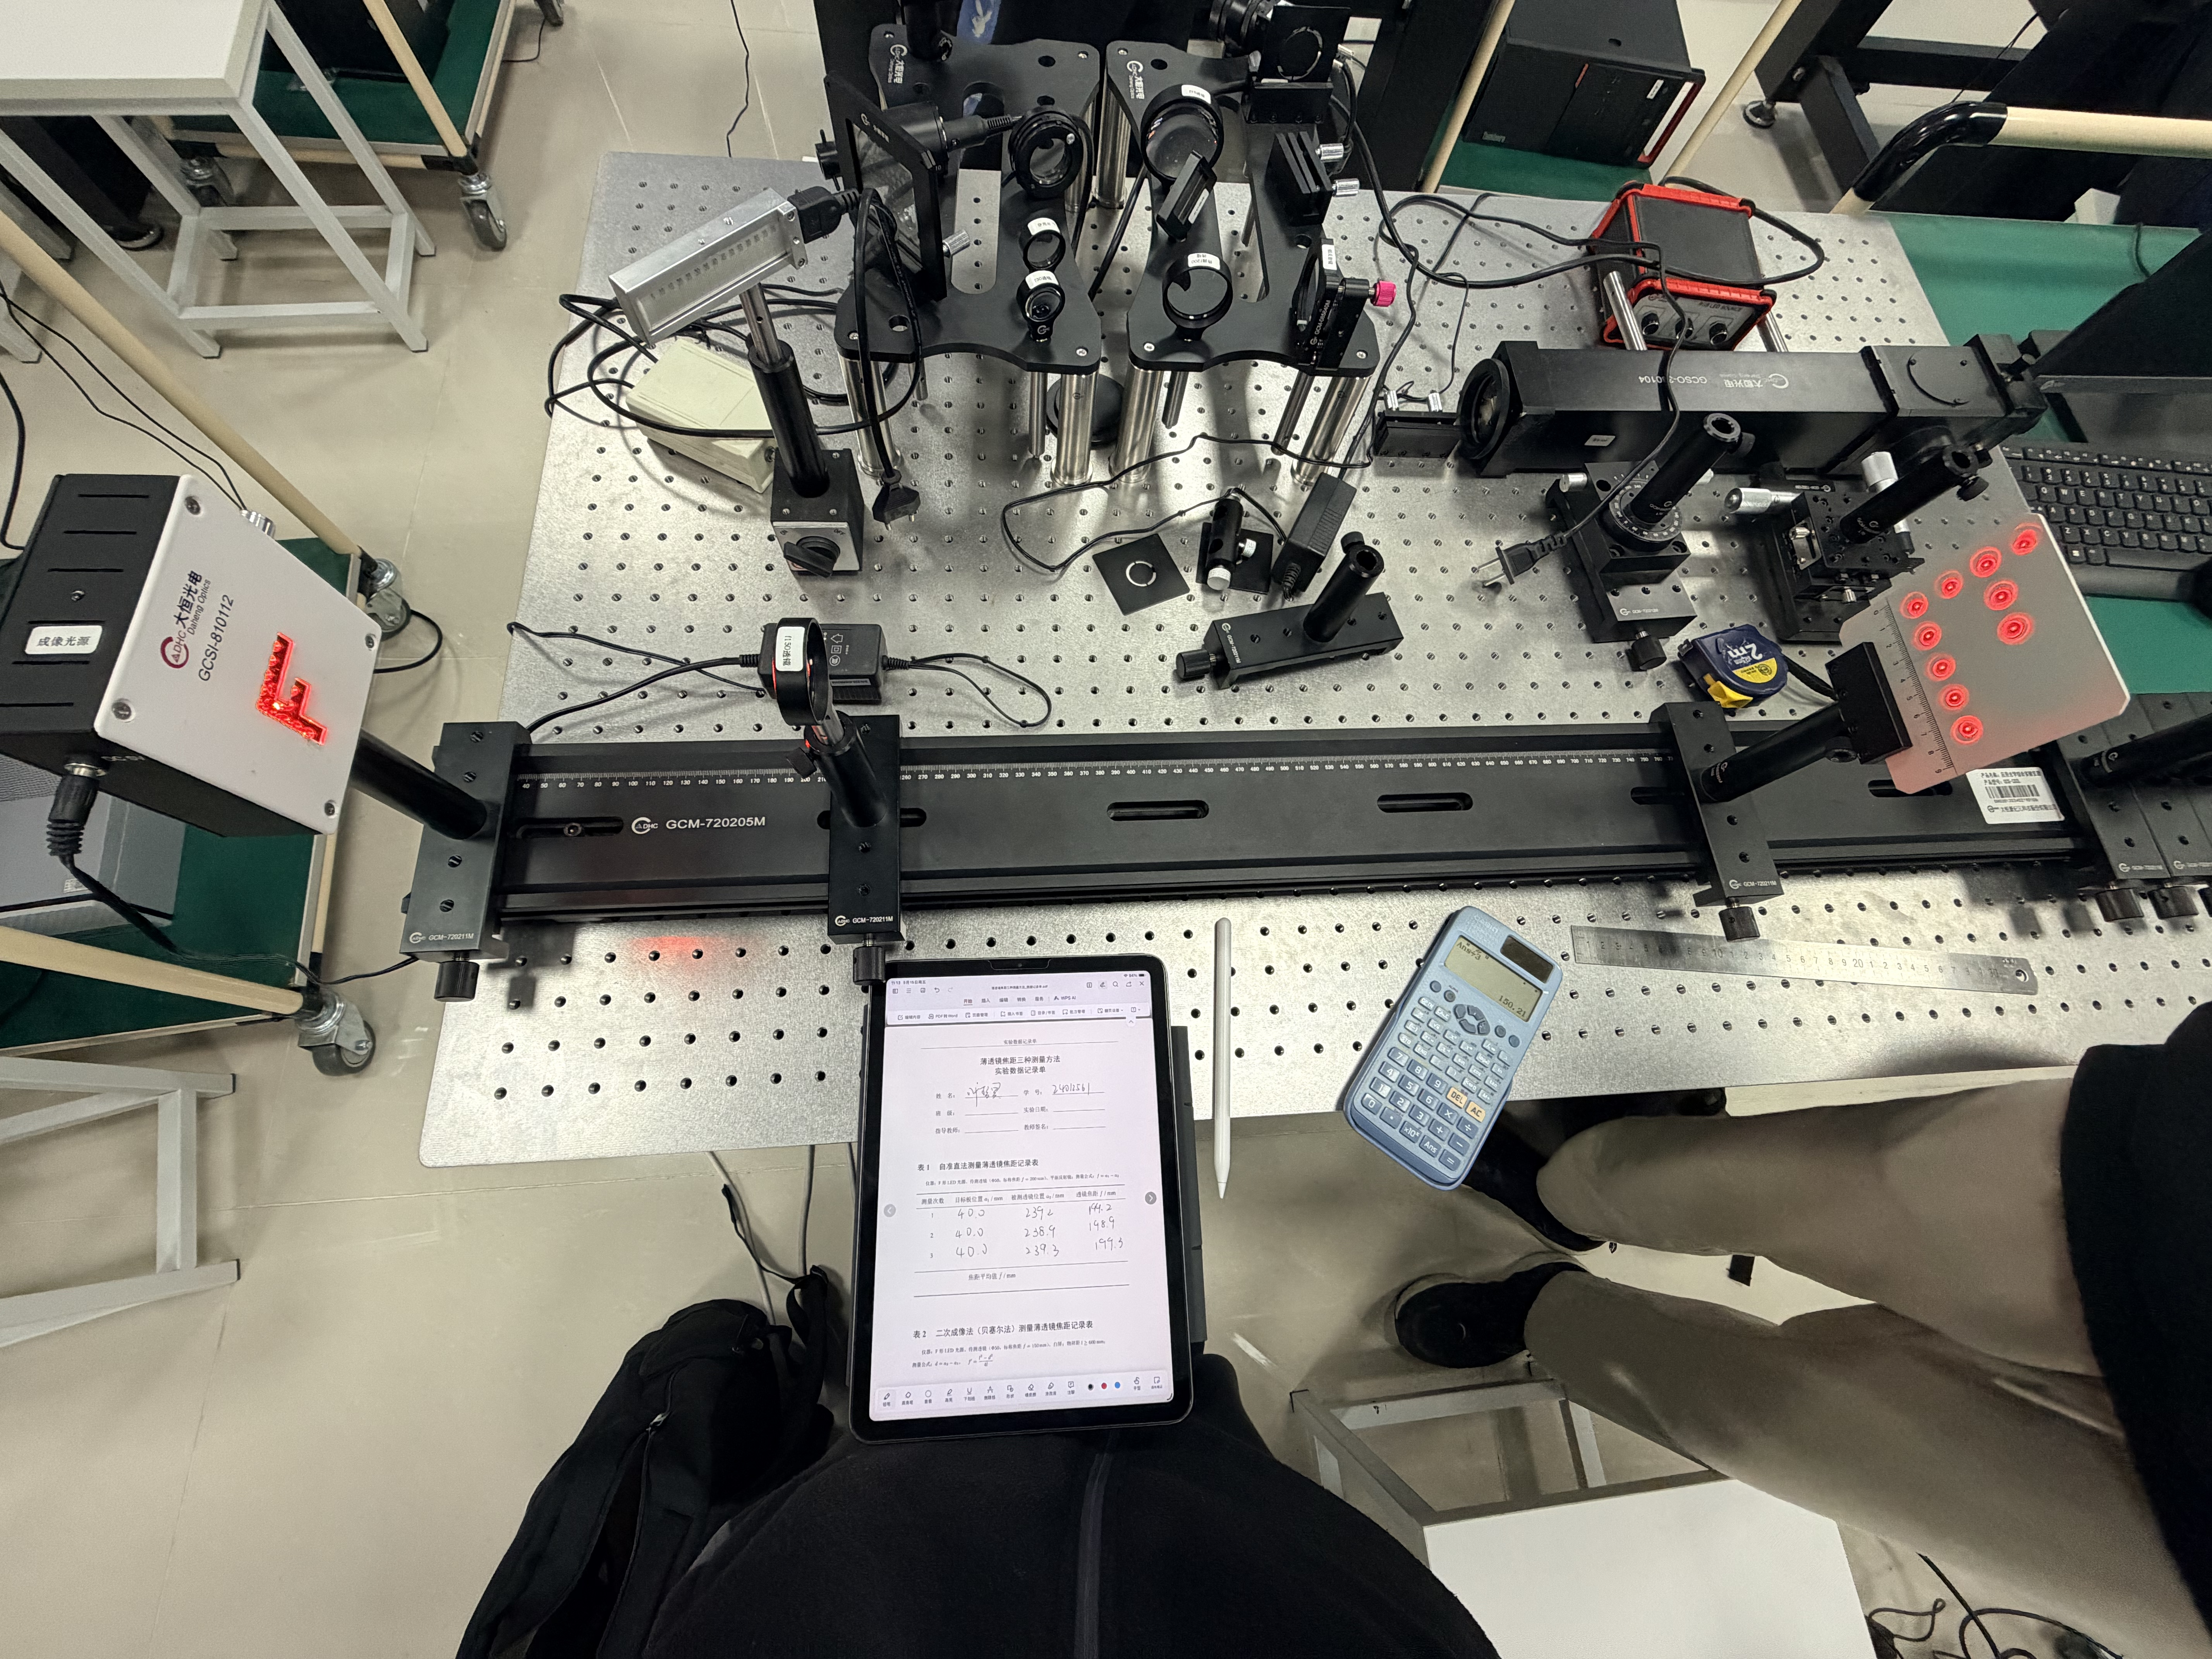
\includegraphics[width=\textwidth]{实验照片/二次成像法光路照片（a1处）.jpg}
    \caption{二次成像法——第一次清晰成像（$a_1$ 处，实拍）}
    \label{fig:bessel-a1}
  \end{minipage}
  \hfill
  \begin{minipage}[b]{0.48\textwidth}
    \centering
    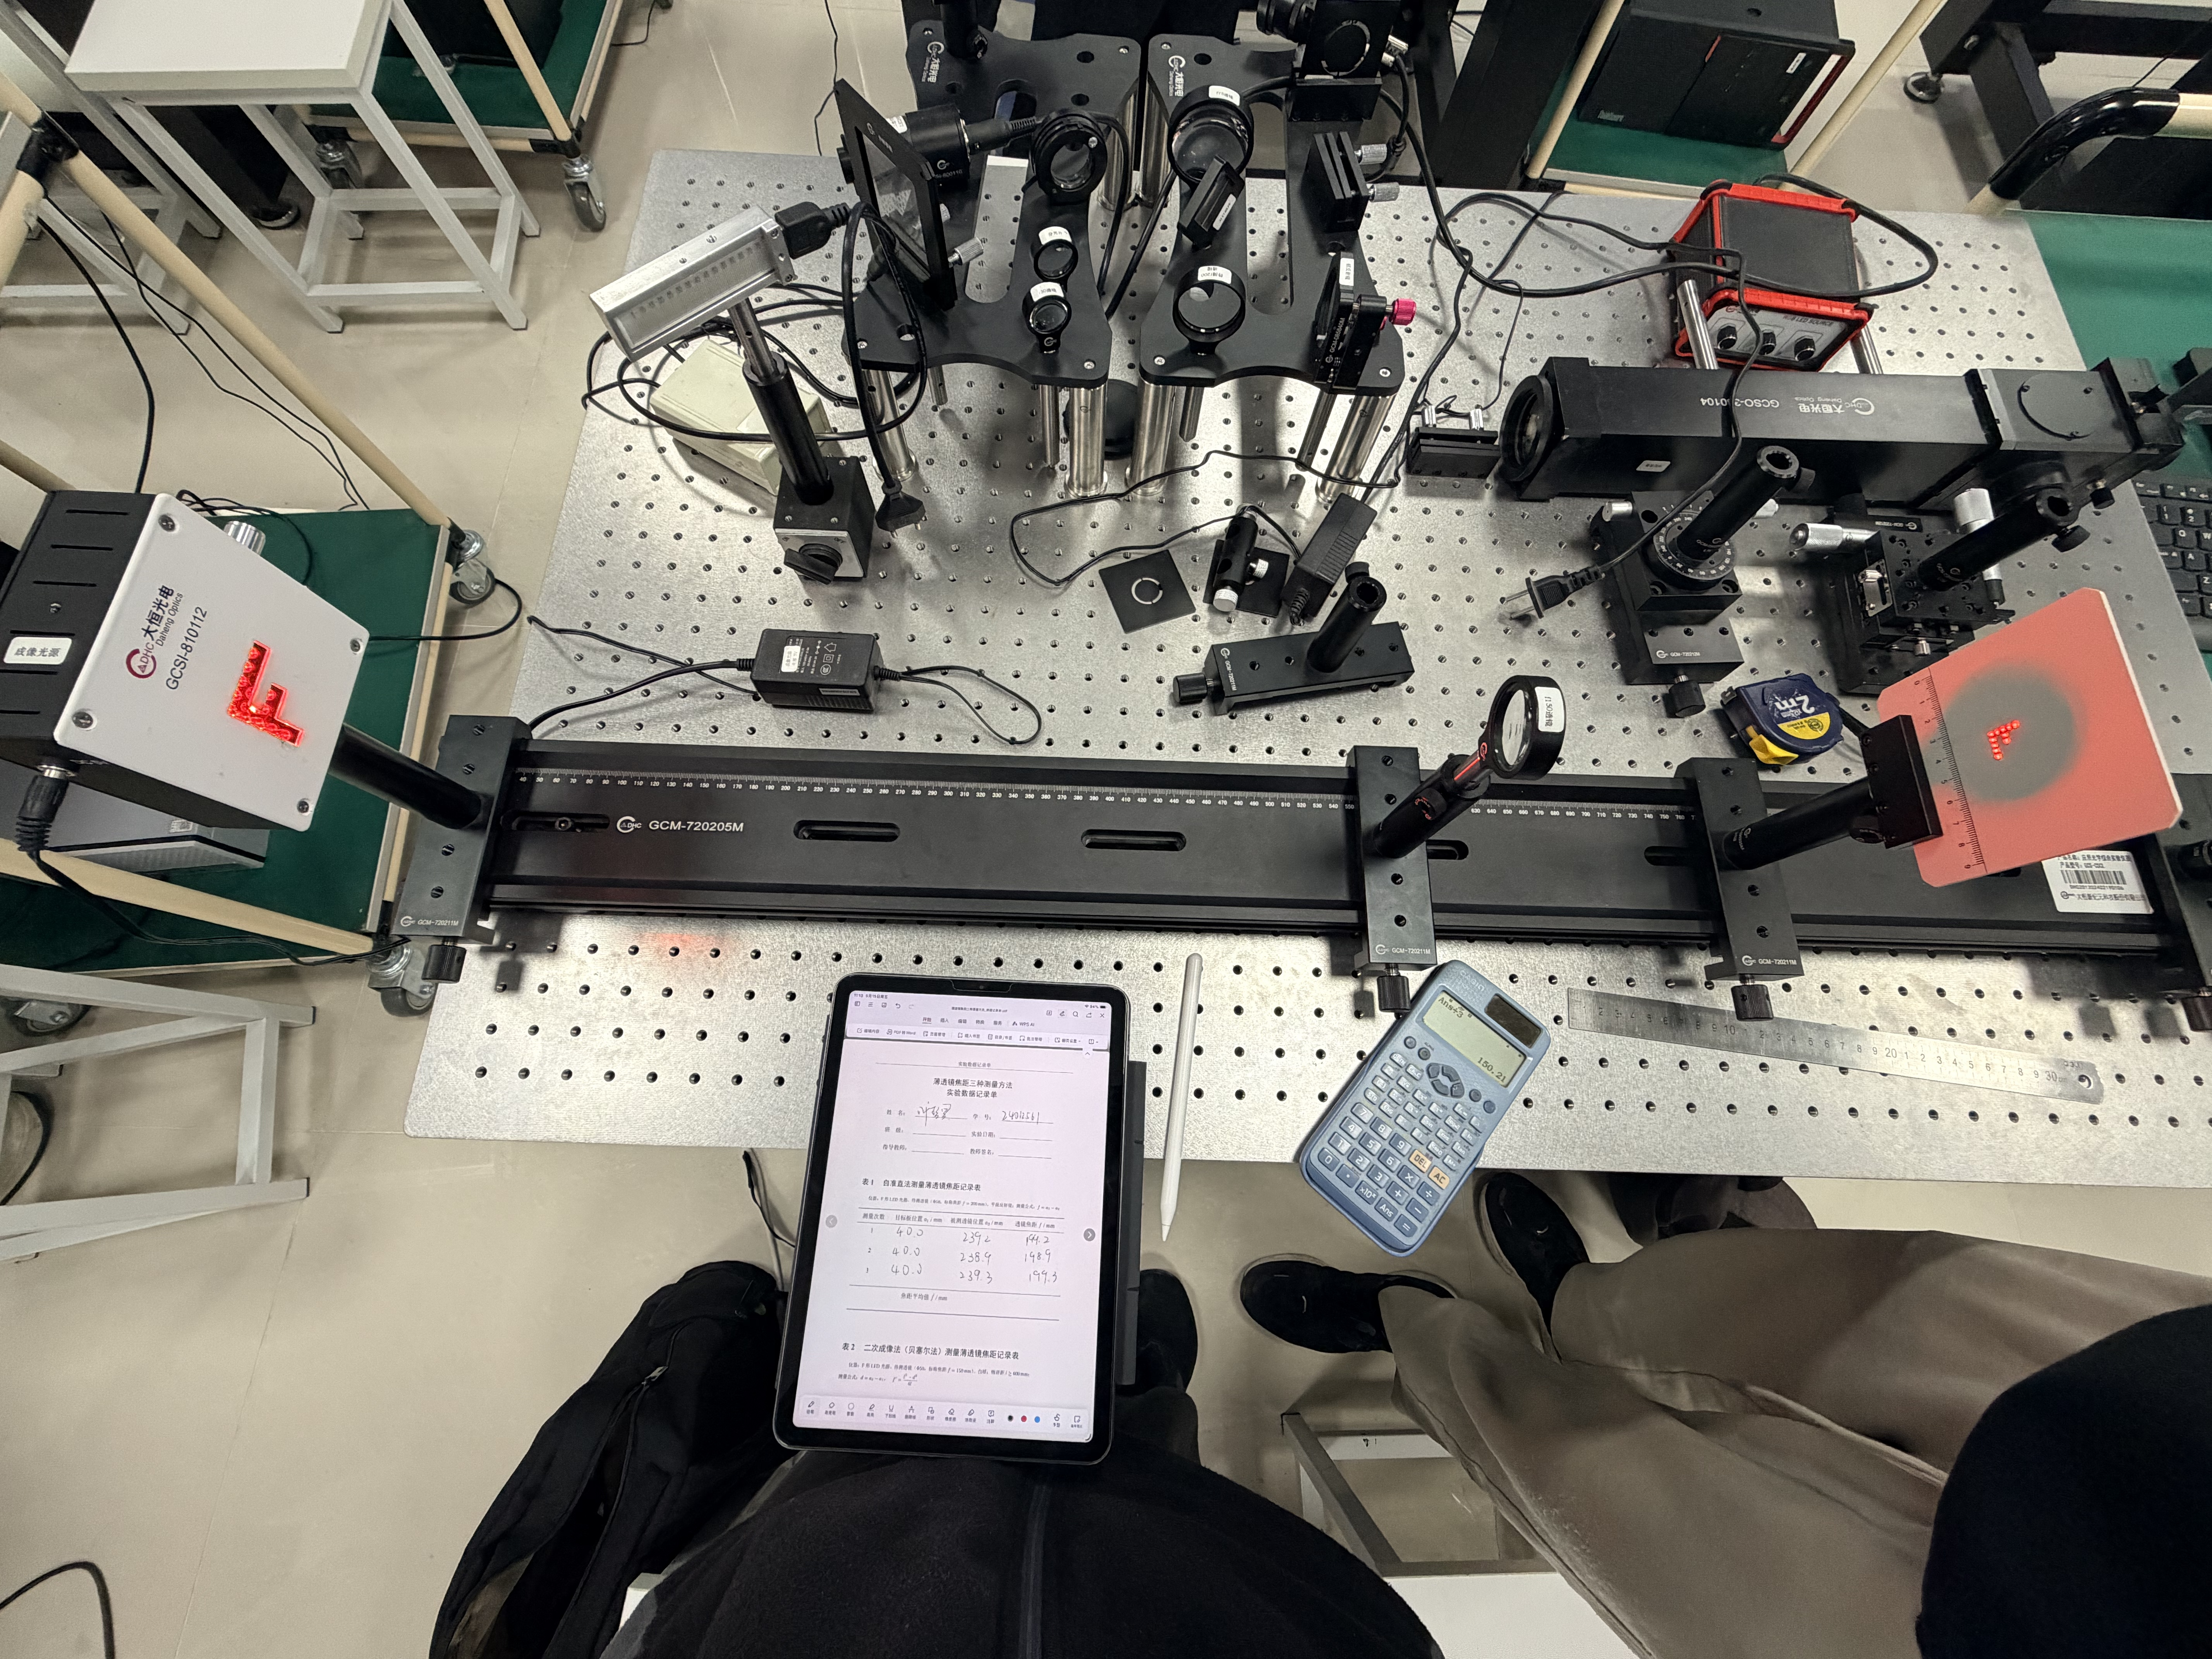
\includegraphics[width=\textwidth]{实验照片/二次成像法光路照片（a2处）.jpg}
    \caption{二次成像法——第二次清晰成像（$a_2$ 处，实拍）}
    \label{fig:bessel-a2}
  \end{minipage}
\end{figure}

% ========== 第 5 节：实验数据与处理 ==========
\section{实验数据与处理}

\subsection{自准直法}

待测透镜标称焦距 $f = 200\,\text{mm}$，测量公式：$f = a_2 - a_1$（透镜位置减目标板位置）。

\begin{table}[H]
  \centering
  \caption{自准直法测量薄透镜焦距记录表}
  \label{tab:zizhi}
  \begin{adjustbox}{max width=\textwidth}
    \begin{tabular}{>{\centering\arraybackslash}m{2cm}
                    >{\centering\arraybackslash}m{4.5cm}
                    >{\centering\arraybackslash}m{4.5cm}
                    >{\centering\arraybackslash}m{3.5cm}}
      \toprule
      测量次数 & 目标板位置 $a_1$ / mm & 透镜位置 $a_2$ / mm & 焦距 $f$ / mm \\
      \midrule
      1 & 40.0 & 239.2 & 199.2 \\[0.4cm]
      2 & 40.0 & 238.9 & 198.9 \\[0.4cm]
      3 & 40.0 & 239.3 & 199.3 \\[0.4cm]
      \midrule
      \multicolumn{3}{c}{焦距平均值 $\bar{f}$ / mm} & 199.1 \\[0.4cm]
      \bottomrule
    \end{tabular}
  \end{adjustbox}
\end{table}

各次焦距值的计算（以第 1 次为例）：
\begin{equation}
  f_1 = a_2 - a_1 = 239.2 - 40.0 = 199.2\,\text{mm}
\end{equation}

焦距平均值：
\begin{equation}
  \bar{f} = \frac{199.2 + 198.9 + 199.3}{3} = \frac{597.4}{3} \approx 199.1\,\text{mm}
\end{equation}

\subsection{二次成像法（贝塞尔法）}

待测透镜标称焦距 $f' = 150\,\text{mm}$，物屏距 $l \geq 600\,\text{mm}$，测量公式
$d = a_2 - a_1$，$f' = \dfrac{l^2 - d^2}{4l}$。

\begin{table}[H]
  \centering
  \caption{二次成像法（贝塞尔法）测量薄透镜焦距记录表}
  \label{tab:bessel}
  \begin{adjustbox}{max width=\textwidth}
    \begin{tabular}{>{\centering\arraybackslash}m{1.6cm}
                    >{\centering\arraybackslash}m{2.6cm}
                    >{\centering\arraybackslash}m{2.6cm}
                    >{\centering\arraybackslash}m{2.6cm}
                    >{\centering\arraybackslash}m{2.6cm}
                    >{\centering\arraybackslash}m{2.6cm}}
      \toprule
      测量次数 &
      \makecell{$a_1$\\/ mm} &
      \makecell{$a_2$\\/ mm} &
      \makecell{$d = a_2 - a_1$\\/ mm} &
      \makecell{$l$\\/ mm} &
      \makecell{$f'$\\/ mm} \\
      \midrule
      1 & 239.3 & 583.1 & 343.8 & 755.3 & 149.7 \\[0.4cm]
      2 & 270.0 & 421.9 & 151.9 & 643.9 & 152.0 \\[0.4cm]
      3 & 220.0 & 550.9 & 330.9 & 746.3 & 149.9 \\[0.4cm]
      \midrule
      \multicolumn{5}{c}{焦距平均值 $\bar{f}'$ / mm} & 150.5 \\[0.4cm]
      \bottomrule
    \end{tabular}
  \end{adjustbox}
\end{table}

各次焦距值的计算过程（以第 2 次为例，验算）：
\begin{equation}
  f' = \frac{l^2 - d^2}{4l}
     = \frac{643.9^2 - 151.9^2}{4 \times 643.9}
     = \frac{414647.2 - 23073.6}{2575.6}
     \approx 152.0\,\text{mm}
\end{equation}

焦距平均值：
\begin{equation}
  \bar{f}' = \frac{149.7 + 152.0 + 149.9}{3} = \frac{451.6}{3} \approx 150.5\,\text{mm}
\end{equation}

% ========== 第 6 节：误差分析 ==========
\section{误差分析}

\subsection{自准直法的偶然误差}

三次测量结果的样本标准差：
\begin{equation}
  s_1 = \sqrt{\frac{(199.2-199.1)^2+(198.9-199.1)^2+(199.3-199.1)^2}{2}}
       = \sqrt{\frac{0.01+0.04+0.04}{2}} \approx 0.2\,\text{mm}
\end{equation}

与标称值的相对误差：
\begin{equation}
  \delta_1 = \frac{|199.1-200|}{200}\times100\% = 0.45\%
\end{equation}

三次测量中目标板固定（$a_1 = 40.0\,\text{mm}$），透镜位置读数高度一致（$a_2$ 变化范围仅
$0.4\,\text{mm}$），说明自准直法在本次实验中重复性良好。

\subsection{二次成像法的偶然误差}

以三次测量结果计算样本标准差：

\begin{equation}
  s = \sqrt{\frac{\sum_{i=1}^{3}(f_i' - \bar{f}')^2}{n-1}}
    = \sqrt{\frac{(149.7-150.5)^2 + (152.0-150.5)^2 + (149.9-150.5)^2}{2}}
\end{equation}
\begin{equation}
  s = \sqrt{\frac{0.64 + 2.25 + 0.36}{2}} = \sqrt{1.625} \approx 1.3\,\text{mm}
\end{equation}

与标称值的相对误差：
\begin{equation}
  \delta = \frac{|\bar{f}' - f_{\text{标称}}|}{f_{\text{标称}}} \times 100\%
          = \frac{|150.5 - 150|}{150} \times 100\% \approx 0.33\%
\end{equation}

\subsection{系统误差来源分析}

\begin{enumerate}
  \item \textbf{导轨刻度读数误差}：导轨刻度精度为 $1\,\text{mm}$，读数存在约 $0.5\,\text{mm}$ 的估读不确定度，
        对 $d$ 和 $l$ 的计算均有影响。
  \item \textbf{成像位置判断误差}：判断"最清晰像"时具有主观性，透镜在一定范围内移动像的变化
        不明显，导致 $a_1$、$a_2$ 的确定存在一定误差。此误差在第 2 次测量中（$d = 151.9\,\text{mm}$）
        可能更为显著，因为两次成像位置之差 $d$ 较小，小幅度的位置误差对 $f'$ 影响较大。
  \item \textbf{薄透镜近似误差}：实验所用透镜具有一定厚度，二次成像法（贝塞尔法）的推导基于
        薄透镜假设，实际厚度带来微小的系统误差，但本方法不依赖透镜主平面位置，此项影响
        较小。
  \item \textbf{共轴调节误差}：若各元件未严格共轴，像会偏离光轴中心，成像的清晰程度判断出现
        偏差，影响 $a_1$、$a_2$ 的读取。
\end{enumerate}

综合来看，两种方法测量结果均与标称值吻合良好：自准直法相对误差 $0.45\%$，二次成像法相对误差 $0.33\%$，结果可靠。

% ========== 第 7 节：实验结论 ==========
\section{实验结论}

\begin{enumerate}
  \item 采用\textbf{自准直法}对标称焦距 $200\,\text{mm}$ 的薄凸透镜进行三次测量，
        得到焦距平均值 $\bar{f} = 199.1\,\text{mm}$，与标称值的相对误差仅 $0.45\%$，
        三次读数重复性良好（极差仅 $0.4\,\text{mm}$），测量结果可靠。
  \item 采用\textbf{二次成像法（贝塞尔法）}对标称焦距 $150\,\text{mm}$ 的薄凸透镜进行三次测量，
        得到焦距平均值 $\bar{f}' = 150.5\,\text{mm}$，与标称值的相对误差仅 $0.33\%$，
        测量结果良好。
  \item \textbf{平行光管法}因设备原因未能实施。
  \item 通过本次实验，掌握了光学导轨的使用方法、共轴调节技巧，加深了对薄透镜成像规律
        （尤其是物像共轭对称性）的理解。
\end{enumerate}

% ========== 第 8 节：思考题 ==========
\section{思考题}

\subsection*{思考题 1：画出测薄透镜焦距三种方法的光路图}

三种方法的光路图如下：

\textbf{（1）自准直法}光路：LED 光源（物体）$\longrightarrow$ 凸透镜 $L$（物处于前焦面）
$\longrightarrow$ 平行光束 $\longrightarrow$ 平面反射镜 $M$（全反射）$\longrightarrow$ 平行光束
$\longrightarrow$ 透镜 $L$ $\longrightarrow$ 在前焦面（物面）处成倒立等大实像。
光路示意可参见图~\ref{fig:zizhi-principle}。

\textbf{（2）二次成像法（贝塞尔法）}光路：物 $O$（目标板）$\longrightarrow$ 凸透镜 $L$
（位置 $a_1$ 或 $a_2$）$\longrightarrow$ 白屏（像面）。当物屏距 $l > 4f'$ 时，透镜在
两个不同位置 $a_1$（放大像）和 $a_2$（缩小像）均可在屏上成清晰像。
光路示意可参见图~\ref{fig:bessel-principle}。

\textbf{（3）平行光管法}光路：LED 光源 $\longrightarrow$ 平行光管（分划板置于物镜焦平面，
出射平行光）$\longrightarrow$ 待测凸透镜 $L_x$ $\longrightarrow$ CMOS 相机（在焦面上
采集分划板像）。由像的大小 $y'$ 和平行光管物镜焦距 $f_o'$ 计算 $f_x' = (y'/y) f_o'$。

\subsection*{思考题 2：比较三种方法测量薄透镜焦距的优势与不足}

\begin{itemize}
  \item \textbf{自准直法}：原理简单，操作快捷，仅需读两个位置即可得焦距，适合快速检测
        和现场使用；但判断"等大倒立"像较为主观，且需要平面反射镜配合，长焦距透镜调节
        耗时；同时该方法基于薄透镜近似，对厚透镜有一定系统误差。

  \item \textbf{二次成像法（贝塞尔法）}：利用物像共轭对称性，推导中不涉及主平面位置，
        适用于厚透镜，测量精度较高；但要求物屏距 $l > 4f'$，当焦距较长时需较长导轨；
        判断两次成像清晰度仍有主观因素，且当 $l$ 接近 $4f'$ 时两个成像位置非常接近，
        不易区分。

  \item \textbf{平行光管法}：精度最高，适合计量实验室和工程检测；操作流程规范，借助软件
        自动计算，减少人为误差；但需要价格昂贵的平行光管和 CMOS 相机，对共轴要求严格，
        设备复杂，不适合一般教学快速演示。
\end{itemize}

% ========== 附录：原始数据记录 ==========
\appendix
\renewcommand{\thefigure}{\Alph{section}-\arabic{figure}}
\renewcommand{\thetable}{\Alph{section}-\arabic{table}}
\section{原始数据记录}

\begin{figure}[H]
  \centering
  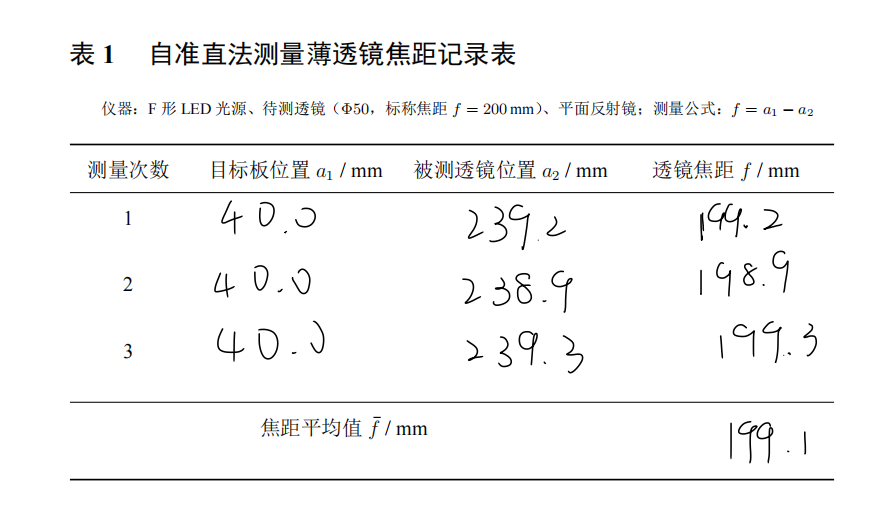
\includegraphics[width=0.85\textwidth]{实验照片/自准直法实验数据记录单.png}
  \caption{原始数据记录——自准直法测量薄透镜焦距记录单（表 1）}
  \label{fig:raw-zizhi}
\end{figure}

\begin{figure}[H]
  \centering
  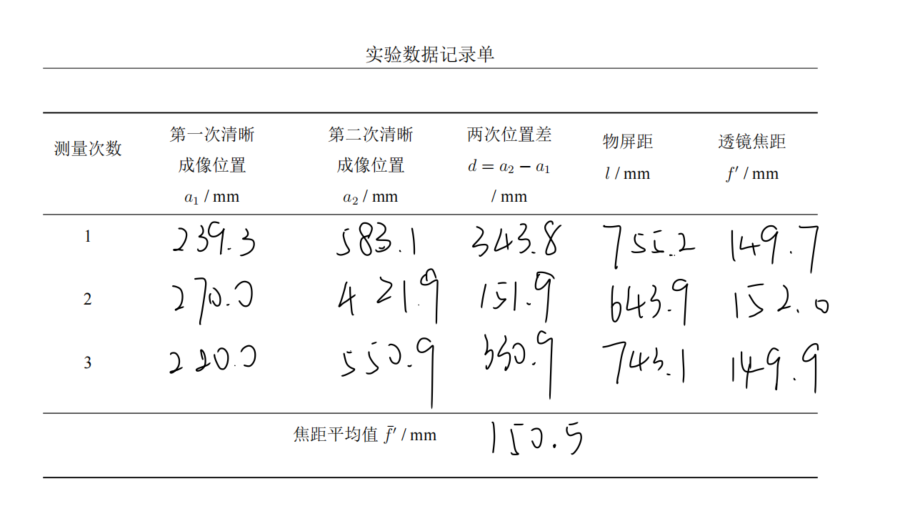
\includegraphics[width=0.85\textwidth]{实验照片/二次成像法实验数据记录单.png}
  \caption{原始数据记录——二次成像法（贝塞尔法）测量薄透镜焦距记录单（表 2）}
  \label{fig:raw-bessel}
\end{figure}

\end{document}
